\section{Vulnerability fixing}

At this point, a corrected version of the code fragment (see subsection \ref{app:C}) is produced by removing the security vulnerabilities found.

Here follows a summary of the vulnerability and flaw analysis performed in section \ref{sec:analysis}:
\begin{description}[itemsep=1.5pt]
    \item[1) vulnerability at line 52:] 'buffer' size is not large enough to receive the copy of 'foo';
    \item[2) flaws at multiple lines:] return values should be checked;
    \item[3) flaws at multiple lines:] errors should be handled;
    \item[4) flaws at multiple lines:] deprecated/unsafe string functions should be replaced by more robust or secure ones;
    \item[5) flaws at multiple lines:] memory management should be done properly;
    \item[6) flaws at multiple lines:] explicit type casting should be performed.
\end{description}

In practice, these latter are fixed in such a way:
\begin{description}[itemsep=1.5pt]
    \item[1), 2), 4):] 'strcpy' at line 52 is replaced by 'StringCbCopyA'\parencite{stringcbcopya} and a return value check is performed;
    \item[2):] a return value check is performed on 'printf' at line 12;
    \item[2):] a return value check is performed on 'fgets' at line 13;
    \item[2), 4):] 'strncpy' at line 18 is replaced by 'StringCbCopyA' and a return value check is performed;
    \item[2), 4):] 'strcat' at line 19 is replaced by 'StringCbCatA'\parencite{stringcbcata} and a return value check is performed;
    \item[2):] return value checks are performed on 'read' at lines 27, 29, 37, 45;
    \item[2), 5):] 'malloc' at lines 28, 44, 50 are replaced by 'calloc', return value checks are performed and memory is eventually deallocated using 'free';
    \item[2):] 'strlen' at line 54 (as argument of 'func3') is replaced by 'strnlen'\parencite{strnlen};
    \item[3):] in case of error (at lines 12, 13, 18, 19, 27, 28, 29, 37, 40, 44, 45, 50, 52), 'exit'\parencite{exit} is called ('EXIT\_FAILURE' is passed as argument);
    \item[6):] explicit type casting is performed ('isalpha' argument to 'unsigned char' at line 15 and 'calloc' return value to 'char *' at lines 28, 44).
\end{description}

Eventually, some minor corrections are made, for instance 'perror' is used to show messages on some standard errors (e.g., on 'read').

Please note that other message errors are not explicitly showed on 'stderr'\parencite{stdin} using 'fprintf', for the sake of brevity.
Moreover, neither a return value check is performed nor possible errors are handled on 'fprintf' at line 40 (this invocation works, in itself, as an error handler).

Now, running \textit{flawfinder} on the "fixed" code fragment using the flag '-m 0' or '--minlevel=0' (and ignoring the warnings that do not represent actual vulnerabilities by adding '// flawfinder: ignore' at the end of the involved lines in the code fragment) shows that all the vulnerabilities found have been removed, as can be seen from figure \ref{fig:final_results_and_analysis_summary_fixed}.
 \begin{figure}[H]
    \centering
    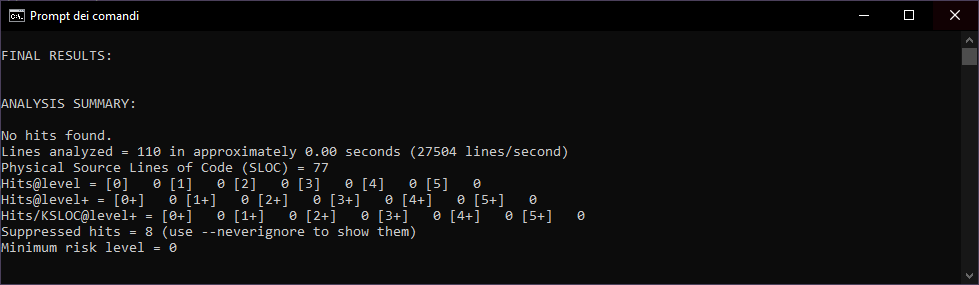
\includegraphics[width=0.9\textwidth]{Resources/final_results_and_analysis_summary_fixed.PNG}
    \caption{final results and summary of the analysis of the fixed code fragment (subsection \ref{app:C})}
    \label{fig:final_results_and_analysis_summary_fixed}
\end{figure}
